%http://texblog.org/2011/09/09/10-ways-to-customize-tocloflot/

%Автоматически вписывать картинки в ширину страницы:
%\includegraphics[maxwidth=\linewidth]{foobar}

\if 0
Так можно сделать многострочный комментарий.
Это маленький хак. Его надо использовать.
\fi

\documentclass[twoside,11pt,a4paper,notitlepage]{report}

\makeatletter
\newcommand*{\toccontents}{\@starttoc{toc}}
\usepackage{pscyr}
\usepackage[T2A]{fontenc}
\usepackage[utf8]{inputenc}
\renewcommand{\rmdefault}{CMR}
\usepackage[russian]{babel}
\usepackage[dvipsnames]{xcolor}

%\usepackage{classicthesis}
%\usepackage[toctitles]{titlesec}
\usepackage{listings}

\usepackage{titlesec}



% Создание индекса
%\usepackage{makeidx}
%\makeindex

%История изменений
%\usepackage{vhistory}
\usepackage[owncaptions]{vhistory}%[tocentry] включить в оглавление


\usepackage[most]{tcolorbox} % для управления цветом
\definecolor{block-gray}{gray}{0.90} % уровень прозрачности (1 - максимум)
\newtcolorbox{myquote}{colback=block-gray,grow to right by=-10mm,grow to left by=-10mm,
	boxrule=0pt,boxsep=0pt,breakable} % настройки области с изменённым фоном

%*************************
\usepackage{shorttoc}% Краткое оглавление
%*************************

%*************************
\usepackage{tocloft}% Управление оглавлением
%*************************



%Fncychar позволит выбрать несколько различных стилей, красиво оформляющих наименование глав.
%\usepackage[Glenn]{fncychap} % выбираем стиль Glenn

%Пакет titlesec позволяет вносить изменения в стандартный стиль главы, то есть переопределять его.
%\usepackage{titlesec, blindtext, color} % подключаем нужные пакеты
%\definecolor{gray75}{gray}{0.75} % определяем цвет
%\newcommand{\hsp}{\hspace{20pt}} % длина линии в 20pt
%% titleformat определяет стиль
%\titleformat{\chapter}[hang]{\Huge\bfseries}{\thechapter\hsp\textcolor{gray75}{|}\hsp}{0pt}{\Huge\bfseries}

\usepackage{listings}      % для кусков программ 
% (понимает синтаксис некоторых языков, чума просто)
\usepackage{alltt}         % для того же
\usepackage{amssymb}       % прикольно для формул

\pagestyle{plain} % нумерация страниц вкл.

%http://tex.stackexchange.com/questions/181183/combine-usepackagetimes-and-fontspec-setmainfont
%http://andreyolegovich.ru/PC/LaTeX.php#base

%********************
% Набор предоставляет дополнительные математические символы, множество удобных возможностей для оформления математических формул (например, упрощённую работу с многострочными формулами) и используется почти во всех LaTeX-документах, в которых есть сколько-нибудь сложные формулы.
%******************** 
\usepackage{amsmath}



\usepackage{titlesec}
\usepackage{csquotes} % ещё одна штука для цитат

\usepackage{sectsty}
%\subsectionfont{\Large\underline}
\subsectionfont{\Large}

\usepackage{graphicx}
\usepackage{sidecap}
\usepackage{xcolor}
\usepackage{pdfpages}
\usepackage{comment}
\usepackage{textcomp}
\usepackage{wrapfig}
\usepackage{sectsty}
\usepackage{lipsum}
\usepackage{fancyhdr}
\usepackage{datetime}
\chapterfont{\centering}

\usepackage{caption}
\usepackage{subcaption}

\usepackage[T2A]{fontenc}
\usepackage{lscape}
\usepackage{makecell}
\usepackage{multicol}
\usepackage{floatrow}
\usepackage{float}
\usepackage{caption}
\usepackage{lastpage} % Allows referencing of the last page to allow footer to read: "Page [Current page] of [Total number of pages]."

\renewcommand{\familydefault}{\sfdefault} %Изменит стандартный шрифт документа на сансерифный.

\definecolor{MSBlue}{rgb}{.204,.353,.541}
\definecolor{MSLightBlue}{rgb}{.31,.506,.741}
%\titleformat*{\section}{\Large\bfseries\sffamily\color{MSBlue}}
%\titleformat*{\subsection}{\large\bfseries\sffamily\color{MSLightBlue}}
%\titleformat*{\subsubsection}{\itshape\subsubsectionfont}

\titleformat
{\chapter} % command
[display] % shape
{\bfseries\Large\itshape} % format
{Story No. \ \thechapter} % label
{0.5ex} % sep
{
	\rule{\textwidth}{1pt}
	\vspace{1ex}
	\centering
} % before-code
[
\vspace{-0.5ex}%
\rule{\textwidth}{0.3pt}
] % after-code


\titleformat{\section}[wrap]
{\normalfont\bfseries}
{\thesection.}{0.5em}{}

\titlespacing{\section}{12pc}{1.5ex plus .1ex minus .2ex}{1pc}





%*****************************************************
% Часто требуется, чтобы номер рисунка содержал в себе номер главы (вроде Рис. 1.1). Чтобы была сделана нумерация по главам, достаточно изменить счётчик рисунков в преамбуле документа вот так:
\renewcommand{\thefigure}{\thesection.\arabic{figure}}
%*****************************************************

%*****************************************************
%Если вас не устраивает вид подрисуночной подписи (например, вместо "Рис. 1:" необходимо "Рис. 1 --- "), используйте пакет caption. В частности, для установки тире в качестве разделителя, вставьте в преамбулу документа следующий код: 
\RequirePackage{caption}
\DeclareCaptionLabelSeparator{defffis}{ --- }
\captionsetup{justification=centering,labelsep=defffis}
%*****************************************************

%\usepackage[colorlinks=true,linkcolor=blue]{hyperref}

%*****************************************************
%Как сделать, чтобы уравнения нумеровались независимо по главам в LaTeX?
%В преамбуле
\makeatletter \@addtoreset{equation}{section} \makeatother 
\makeatletter \@addtoreset{figure}{section} \makeatother 
%*****************************************************

\addto\captionsrussian{
	\def\figurename{Рисунок}
}


\usepackage[hypcap]{caption}

%*****************************************************
% Начинать секции с новой страницы
\usepackage{titlesec}
\newcommand{\sectionbreak}{\clearpage}
%*****************************************************


%*****************************************************
%Чтобы в генерированном PDF работали гиперссылки, то надо подключить модуль hyperref (и если хотите их разрисовать, то модуль по работе с цветами xcolor):
\usepackage{hyperref}
% Цвета для гиперссылок
\definecolor{linkcolor}{HTML}{012b37} % цвет ссылок
\definecolor{urlcolor}{HTML}{012b37} % цвет гиперссылок
\hypersetup{pdfstartview=FitH,  linkcolor=linkcolor,urlcolor=urlcolor, colorlinks=true}
%*****************************************************

%***************************************************** 
%Для удаления номеров страниц из \listoffigures
\makeatletter
\newcommand{\emptypage}[1]{%
	\cleardoublepage
	\begingroup
	\let\ps@plain\ps@empty
	\pagestyle{empty}
	#1
	\cleardoublepage}
\makeatletter
%*****************************************************


\setcounter{secnumdepth}{3}
%\usepackage{enumitem}
\usepackage[shortlabels]{enumitem}
\setlist[enumerate]{leftmargin=*,align=left,label=\thesubsection.\arabic*.}
%\usepackage{enumerate}
\usepackage{longtable}

%\renewcommand{\rmdefault}{ftm}
\renewcommand{\rmdefault}{cmr}
\renewcommand{\thesection}{\arabic{section}}
%\usepackage{enumitem}
%%% Страница
%\usepackage{extsizes} % Возможность сделать 14-й шрифт
\usepackage{geometry} % Простой способ задавать поля
\geometry{top=15mm}
\geometry{bottom=10mm}
\geometry{left=10mm}
\geometry{right=10mm}

%*****************************************************
%Here is how you can increase the space between the number and the caption in your \listoffigures. Add the following two lines before your \begin{document}:
\usepackage{tocloft}
\setlength{\cftfignumwidth}{3em}
%With the tocloft-package you can control the design of table of contents, figures and tables.
%*****************************************************

% раскомментировать, чтобы увидеть забавную картинку размещения текста
%\usepackage{layout}
% увидеть, что не сработало и раскомментировать \layout внизу
%%%%%%%%%%%%%%%%%%%%%%%%%%%%%%%%%%%%%%%%%%%%%%%%%%%%%%%%%%%%%%%%%%%%%%%%%%%%%%%%


%%%%%%%%%%%%%%%%%%%%%%%%%%%%%%%%%%%%%%%%%%%%%%%%%%%%%%%%%%%%%%%%%%%%%%%%%%%%%%%%
%%%
%%% мелочи жизни (переопределение буллетов для списков)
%%%
\renewcommand{\labelitemii}{{$\mathbf{+}$}}
\renewcommand{\labelitemiii}{{$\mathbf{++}$}}

%%%%%%%%%%%%%%%%%%%%%%%%%%%%%%%%%%%%%%%%%%%%%%%%%%%%%%%%%%%%%%%%%%%%%%%%%%%%%%%%
%%%
%%% Моя любимая настройка параметров страницы. По умолчанию колонка узковатая
%%%
\voffset=-10mm
\topmargin=0mm
\headheight=5mm
\headsep=10mm

\textheight=237mm
\footskip=10mm

\oddsidemargin=-2mm
\evensidemargin=-15mm
% регулирует расстояние sidenotes от края страницы
\hoffset=5mm
\textwidth=175mm
\marginparsep=10mm
%%%%%%%%%%%%%%%%%%%%%%%%%%%%%%%%%%%%%%%%%%%%%%%%%%%%%%%%%%%%%%%%%%%%%%%%%%%%%%%%

\usepackage{caption}

\usepackage{svn}


\pagestyle{fancy}
%\fancyfoot[]{вер. 1.05}

%\fancyhead[C]{Страница \thepage \; из \pageref{LastPage}}
%\fancyhead[RE]{\slshape\nouppercase{\rightmark}}
%\fancyhead[LO]{\slshape\nouppercase{\leftmark}}
%\fancyfoot[C]{Страница \thepage \; из \pageref{LastPage}}
%\renewcommand{\headrulewidth}{0pt}
%\renewcommand{\footrulewidth}{0pt}
%\lhead{\footnotesize \parbox{11cm}{Draft 1} }

% Allows calling chapter and section names in headers and footers.
%\renewcommand{\chaptermark}[1]{%
%	\markboth{\chaptername\ \thechapter}
%	{\noexpand\firstsubsectiontitle}}
%\renewcommand{\sectionmark}[1]{}
%\renewcommand{\subsectionmark}[1]{%
%	\markright{#1}\gdef\firstsubsectiontitle{#1}}
%\newcommand\firstsubsectiontitle{}



\lhead{\footnotesize \parbox{11cm}}
%\lfoot{\footnotesize \parbox{11cm}{\textit{2}}}
%\cfoot{}
\rhead{\footnotesize  \chaptername \ - \rightmark}
%\rfoot{\footnotesize Page \thepage\ of \pageref{LastPage}}
%\fancyfoot[C]{Страница \thepage \; из \pageref{LastPage}}
\fancyfoot{} % Clear all footer fields
\fancyfoot[RO,L] {v.\vhCurrentVersion \ \vhCurrentDate}  % Версия и дата
\fancyfoot[RO,R]{Страница \thepage \; из \pageref{LastPage}} % Page number on right in footer

%\renewcommand{\headheight}{24pt}
\setlength{\headheight}{4pt}
\renewcommand{\footrulewidth}{0pt}
%\setlength\headheight{80.0pt}
%\addtolength{\textheight}{-80.0pt}
%\chead{\includegraphics[width=\textwidth]{img/log1o.png}}
%\cfoot{\includegraphics[width=\textwidth]{img/foot.png}}

\graphicspath{{images/}}



%*****************************************************
%Номера страниц, включающие номер главы
\usepackage[auto]{chappg} %%% this is to set the page numbers as Chapter-Page.
%*****************************************************



\newdate{date}{28}{01}{2016}
\date{\displaydate{date}}
%Increase the value of tocdepth and secnumdepth. The tocdepth value determines to which level the sectioning commands are printed in the ToC (they are always included in the .toc file but ignored otherwise). The secnumdepth value determines up to what level the sectioning titles are numbered. They are LaTeX counters and you can set them using 
\setcounter{tocdepth}{1}
\setcounter{secnumdepth}{4}

\renewcommand{\theenumi}{\arabic{enumi}}
\renewcommand{\labelenumi}{\arabic{enumi}}
\renewcommand{\theenumii}{.\arabic{enumii}}
\renewcommand{\labelenumii}{\arabic{enumi}.\arabic{enumii}.}
\renewcommand{\theenumiii}{.\arabic{enumiii}}
\renewcommand{\labelenumiii}{\arabic{enumi}.\arabic{enumii}.\arabic{enumiii}.}


\usepackage{titlepic}



%\titlespacing\section{0pt}{12pt plus 4pt minus 2pt}{0pt plus 2pt minus 2pt}
%\titlespacing{\subsection}{0pt}{\parskip}{-\parskip}

\def\capfigure{figure}

\def\captable{table}

\long\def\@makecaption#1#2{%
	
	\vskip\abovecaptionskip
	
	\ifx\@captype\capfigure
	
	\centering #1~--~#2 \par
	
	\else
	
	#1~--~#2 \par
	
	\fi
	
	\vskip\belowcaptionskip}

\setlength\abovecaptionskip{2\p@}

\setlength\belowcaptionskip{1\p@}



%%%%%%%%%%%%%%%%%%%%%%%%%%%%%%%%%%%%%%%%%%%%%%%%%%%%%%%%%%%%%%%%%%%%%%%%%%%%%%%%
%%%
%%% маленький хак, новое окружение 'algorithm' (см. использование ниже)
%%%
\newlength{\algboxsp}
\setlength{\algboxsp}{2mm}
\newsavebox{\algbox}
\newenvironment{basealgorithm}
{\begin{lrbox}{\algbox}\begin{minipage}{\textwidth}\begin{alltt}}
			{\end{alltt}\end{minipage}\end{lrbox}
	\fbox{
		\parbox{0.95\textwidth}{
			\makebox[0mm]{}
			\\[\algboxsp]
			\mbox{\hspace{\algboxsp}}
			\usebox{\algbox}
			\\[\algboxsp] } }}

\newenvironment{algorithm}[1]
{\begin{figure}[btp]\def\algcptn{\caption{#1}}\begin{basealgorithm}}
		{\end{basealgorithm}\algcptn\end{figure}}
	
	
	
%**********************************
% Todo notes - example from http://www.texample.net/tikz/examples/todo-notes/
\usepackage{verbatim}
\usepackage[colorinlistoftodos]{todonotes}
%**********************************

%\usepackage{sidenotes}


\usepackage{geometry}

\usepackage{snotez}



%**********************************************************

% Vertically aligning a marginnote and a section title
%**********************************************************
\usepackage{lipsum}

\usepackage{marginnote}
\reversemarginpar % To put the margin pars on the left
\renewcommand*{\marginfont}{\normalfont\normalsize}

\usepackage{tikz}
\usetikzlibrary{calc}
\usetikzlibrary{backgrounds}

\newcommand*{\Date}[4]{%
	\begin{tikzpicture}[show background rectangle,inner frame sep=0pt,text width=1cm,align=center]
	\node [fill=orange] at (0,0)                                (dayofweek)  {#1};
	\node [fill=white ] at ($(dayofweek)  +(0,-\baselineskip)$) (dayofmonth) {#2};
	\node [fill=white ] at ($(dayofmonth) +(0,-\baselineskip)$) (month)      {#3};
	\node [fill=orange] at ($(month)      +(0,-\baselineskip)$) (dayofmonth) {#4};
	\end{tikzpicture}
}

%**********************************************************
\usepackage{geometry}
\usepackage{marginnote}





	
\renewcommand{\cftchapfont}{\scshape}
\renewcommand{\cftsecfont}{\bfseries}
%\renewcommand{\cftfigfont}{Figure }
%\renewcommand{\cfttabfont}{Table }
	
\usepackage{eso-pic}	


\AddToShipoutPicture{%

	\AtPageLowerLeft{%
		\hspace*{.02\textwidth}%
		\rotatebox{90}{%
			\begin{minipage}{\paperheight}
				\fontsize{6}{6}\selectfont
				%				\centering\textcopyright~\today{} ТД Крюгер
					\textcopyright~ ТД Крюгер
	%				\textcopyright~ ТД Крюгер тел.техподдержки 8-913 016 0854
			\end{minipage} %
		}
	} %
}%

%How can I put real notes in the margin?
%**********************************************************	
\usepackage{xparse}
\usepackage{tikz}
\usetikzlibrary{calc,fit, decorations.pathmorphing}

\makeatletter
% http://tex.stackexchange.com/questions/39296/simulating-hand-drawn-lines
\pgfdeclaredecoration{penciline}{initial}{
	\state{initial}[width=+\pgfdecoratedinputsegmentremainingdistance,auto corner on length=1mm,]{
		\pgfpathcurveto%
		{% From
			\pgfqpoint{\pgfdecoratedinputsegmentremainingdistance}
			{\pgfdecorationsegmentamplitude}
		}
		{%  Control 1
			\pgfmathrand
			\pgfpointadd{\pgfqpoint{\pgfdecoratedinputsegmentremainingdistance}{0pt}}
			{\pgfqpoint{-\pgfdecorationsegmentaspect\pgfdecoratedinputsegmentremainingdistance}%
				{\pgfmathresult\pgfdecorationsegmentamplitude}
			}
		}
		{%TO 
			\pgfpointadd{\pgfpointdecoratedinputsegmentlast}{\pgfpoint{1pt}{1pt}}
		}
	}
	\state{final}{}
}
\makeatother
\newcommand{\tikzmark}[1]{\tikz[overlay,remember picture] \node (#1) {};}
\newcommand{\CommentText}[3]{\tikzmark{#1}#3\tikzmark{#2}}
\NewDocumentCommand{\CommentPar}{%
	O{}% #1 = draw options for the referenced word
	O{}% #2 = draw options for the comment
	O{}% #3 = draw options for the connecting line
	m  % #4 = left \tikzmark name
	m  % #5 = left \tikzmark name
	m  % #6 = comment
}{%
	\begin{tikzpicture}[overlay,remember picture,decoration=penciline, thick]
	\node [shape=rectangle,inner sep=0, draw=blue, ,rounded corners=2pt, fit={(#4.south) ($(#5.north)+(0,0.75ex)$)}, decorate, #1] (Source) {};
	\node at ($(#4)!0.5!(#5)$) [blue, font=\itshape, rounded corners=5pt, decorate, #2] (Label) {#6};
	\draw [draw=red, decorate, #3] (Label) to (Source);
	\end{tikzpicture}
}

%**********************************************************
\usepackage[os=win]{menukeys}
% меняестся стиль, тени у кнопок
%**********************************************************
%\changemenucolor{gray}{txt}{named}{red} %Изменение цвета 
\renewmenumacro{\keys}[>]{shadowedroundedkeys}
\renewmenumacro{\menu}{roundedmenus} % default: menus
%\newmenumacro{\button}
%**********************************************************


% белые кнопки вызов \keystroke{Ctrl} 
\newcommand*\keystroke[1]{%
	\tikz[baseline=(key.base)]
	\node[%
	draw,
	fill=white,
	drop shadow={shadow xshift=0.25ex,shadow yshift=-0.25ex,fill=black,opacity=0.75},
	rectangle,
	rounded corners=2pt,
	inner sep=1pt,
	line width=0.5pt,
	font=\scriptsize\sffamily
	](key) {#1\strut}
	;
}

%%%%%%%%%%%%%%%%%%%%%%%%%%%%%%%%%%%%%%%%%%%%%%%%%%%
% Для рамки "Внимание"
%\usepackage{fourier}

\usepackage[utf8]{inputenc}
\usepackage{newunicodechar}

\newcommand\Warning{%
	\makebox[1.4em][c]{%
		\makebox[0pt][c]{\raisebox{.1em}{\small!}}%
		\makebox[0pt][c]{\color{red}\Large$\bigtriangleup$}}}%

\newunicodechar{⚠}{\Warning}



\usepackage{blindtext}
\usepackage{pifont,mdframed}

\newenvironment{warning}
{\par\begin{mdframed}[linewidth=2pt,linecolor=red]%
		\begin{list}{}{\leftmargin=1cm
				\labelwidth=\leftmargin}\item[\Large \Warning]} %				\labelwidth=\leftmargin}\item[\Large\ding{43}]}
		{\end{list}\end{mdframed}\par}

%%%%%%%%%%%%%%%%%%%%%%%%%%%%%%%%%%%%%%%%%%%%%

%%%%%%%%%%%%%%%%%%%%%%%%%%%%%%%%%%%%%%%%%%%%%%%%%%%%%%%%%%%%%%%%%%%%%%%%%%
%How to remove headers and footers for pages between chapters?
\makeatletter
\renewcommand*{\cleardoublepage}{\clearpage\if@twoside \ifodd\c@page\else
	\hbox{}%
	\thispagestyle{empty}%
	\newpage%
	\if@twocolumn\hbox{}\newpage\fi\fi\fi}
\makeatother
%%%%%%%%%%%%%%%%%%%%%%%%%%%%%%%%%%%%%%%%%%%%%%%%%%%%%%%%%%%%%%%%%%%%%%%%%%
% http://tex.stackexchange.com/questions/39017/how-to-influence-the-position-of-float-environments-like-figure-and-table-in-lat
% СЧЕТЧИКИ / COUNTERS
%    totalnumber (default 3) =Макс кол-во флоатс на странице
%                             max number of floats in a page
%    topnumber (default 2) = макс кол-во флоатс вверху страницы
%                            max number of floats in the top area
%    bottomnumber (default 1) = макс кол-во флоатс внизу страницы
%                               max number of floats in the bottom area
% РАЗМЕРЫ (доли страницы) / AREAS (use \renewcommand)
%    \topfraction (default 0.7) макс доля, проходящаяся на верх страницы
%                               maximum size of the top area
%    \bottomfraction (default 0.3)  макс доля приходящаяся на низ
%                                   maximum size of the bottom area
%    \textfraction (default 0.2)  миним доля, которая должна быть занята текстом
%                                 minimum size of the text area, i.e., the area that must not be occupied by floats
%\setlength{\intextsep}{4ex} % remove extra space above and below in-line float
%\setlength{\floatsep }{1ex} % remove extra space above and below in-line float

%% Попробуйте поизменять параметры и понаблюдайте за эффектом
%% Try changing the below parameters to see the effect
%\setcounter{totalnumber}{10}
%\setcounter{topnumber}{10}
%\setcounter{bottomnumber}{10}
%\renewcommand{\topfraction}{1}
%\renewcommand{\bottomfraction}{1}
%\renewcommand{\textfraction}{10}




%\setlength{\abovecaptionskip}{-1pt}
%\setlength{\belowcaptionskip}{-1pt}
%\usepackage[section]{placeins}
%\setlength{\textfloatsep}{5pt plus 1.0pt minus 2.0pt}

\setcounter{totalnumber}{10}
 \setcounter{topnumber}{10}

\renewcommand{\topfraction}{1}
 \renewcommand{\textfraction}{0}

%\setlength{\textfloatsep}{10pt plus 1.0pt minus 2.0pt}
%\setlength{\floatsep}{5pt plus 1.0pt minus 1.0pt}
%\setlength{\intextsep}{5pt plus 1.0pt minus 1.0pt}
\begin{document}
\newcommand{\PK}{Pashkov}
% Расшифровка сокращений для обозначения авторов 
\renewcommand{\vhhistoryname}{Журнал изменений} 
\renewcommand{\vhversionname}{Версия} 
\renewcommand{\vhdatename}{Дата} 
\renewcommand{\vhauthorname}{Автор(ы)} 
\renewcommand{\vhchangename}{Изменения} 

%\layout
\begin{titlepage}
  \begin{center}
    \large
  ООО ТД ,,Крюгер``

 
\vspace{2.25cm}

\textbf{Описание добавлений и изменений в конфигурации 1С Розница} 

\textit{Конфигурация Розница 2.2}
\vfill    
  
{
\includegraphics[width=5cm]{logo.png}}  
  
\end{center}
\vfill

\newlength{\ML}
\settowidth{\ML}{«\underline{\hspace{0.7cm}}» \underline{\hspace{2cm}}}


\begin{center}
  Новосибирск, 2017 г.
\end{center}
\end{titlepage}	
%\newpage	
\setcounter{tocdepth}{3}% Include \subsubsection in ToC 
%## убрали номер страницы с содержания
\cleardoublepage
\pagenumbering{gobble}

%\shorttableofcontents {Краткое оглавление }{1}% Краткое оглавление
\tableofcontents

\addtocontents{toc}{~\hfill\textbf{Стр}\par}
\cleardoublepage
\pagenumbering{arabic}
%#############################
%\newpage	
%
\section{Описание добавлений и изменений в конфигурации 1С Розница}
%\newpage	
\section{Закупки}
%\marginnote{\Date{Ср.}{08}{Апр.}{2020}}[-20pt]
\subsection{Поступление товаров}
\subsubsection{Поступление товаров на основании ТТН Входящей ЕГАИС}



\begin{itemize}
	\item Реквизит "Поставщик" должен быть недоступен для изменения (расш.)
	\Nameref{500}
	\item Реквизиты <<НомерВходящегоДокумента>> <<ДатаВходящегоДокумента>> должны быть недоступны для изменения (расш.)\Nameref{500}
	\item В табличной части <<Товары>> для редактирования доступны только поля:
	<<Цена>>, <<Всего>>, <<\%НДС->>, <<НДС>>.  (расш.)\Nameref{500}
	\item <<галочка>> "Есть расхождения" невидима (расш.)\Nameref{501}
	\item При создании документа на основании Входящей ТТН ЕГАИС в табличной части <<Товары>>
	корректно пересчитывается количество из  декалитров в литры (расш.)\Nameref{501}
	\item При заполнении документа на основании Входящей ТТН ЕГАИС реквизит <<Поставщик>> заполняется из реквизита <<Грузоотправитель>> Входящей ТТН ЕГАИС
	
\end{itemize}

\subsubsection{Поступление товаров общие свойства}

\begin{itemize}
	\item При установленной константе <<крюПроверятьПомеченнуюНаУдалениеВДокументах>>
	документ не должен проводиться, если в табличной части <<Товары>> присутствует 
	номенклатура помеченная на удаление.(описание)\Nameref{1005}
	\item При проведении документ должен делать движения по регистру <<СебестоимостьНоменклатуры>> (описание)\Nameref{1002}
	\item При установленной константе <<крюПроводитьТару>> и наличии в табличной части <<Товары>> номенклатуры
	с видом "Возвратная тара" или <<Оборудование>>, документ должен делать движения по регистру <<ТараНаСкладах>> (описание)\Nameref{1003}
	\item Если табличная часть <<Товары>> содержит алкогольную продукцию, а документ не имеет в основании Входящую ТТН ЕГАИС, то документ не проводится (расш.)\Nameref{500}
	\item Если сумма являющейся основанием Входящей ТТН ЕГАИС не совпадает с суммой документа, то выдается предупреждение с требованием откорректировать суммы (расш.)
	\Nameref{500}
	\item Если в табличной части <<Товары>> есть строки содержащие цены на товар, которые отсутствуют или выше чем те, которые хранятся в регистре <<крюЦеныНоменклатурыКонтрагентов>> по данному поставщику, то проведение документа блокируется, и на назначенные адреса электронной почты уходит письмо с сообщение о данном событии. (расш.)\Nameref{500}
	(описание)\Nameref{1006}
\end{itemize}
\vspace{\baselineskip}\par
\subsubsection{Поступление товаров дополнительные механизмы}
\begin{itemize}
	\item Существует константа <<крюДатаЗапретаПроведенияДокументовБезТранспортнойТары>> при 
	включении которой (установке даты) включается механизм контроля заполнения транспортной тары
	\begin{myquote}
     Необходимо проверить актуальность этого механизма.
	\end{myquote}
	
	
\end{itemize}	



\subsection{Возврат товаров поставщику}
\begin{itemize}
	\item При установленной константе <<крюПроверятьПомеченнуюНаУдалениеВДокументах>>
	документ не должен проводиться, если в табличной части <<Товары>> присутствует 
	номенклатура помеченная на удаление.(описание)\Nameref{1005}
	\item При установленной константе "крюПроводитьТару" и наличии в табличной части
	 Товары номенклатуры	с видом "Возвратная тара" или "Оборудование", документ должен делать движения по регистру "ТараНаСкладах" (описание)\Nameref{1003}
	\item  Регулировка механизма выгрузки в бухгалтерию. На форме добавлены два дополнительных реквизита "крюВыгружатьВБухгалтериюФ" и "крюНЕВыгружатьВБухгалтериюФ" при "включении" одного реквизита второй должен отключаться
	 (расш.)
	 \Nameref{502}
	\item Установленная константа "крюОчищатьНДСВВозвратеПоставщику" очищает признак учета НДС в Возврате поставщику.
	\item При печати ТОРГ-12 в представление организации в шапку добавлен КПП и параметр вид операции-Возврат (модуль менеджера)

\end{itemize}


\subsection{Перемещение товаров}

\begin{itemize}
	\item При установленной константе <<крюПроверятьПомеченнуюНаУдалениеВДокументах>>
	документ не должен проводиться, если в табличной части <<Товары>> присутствует 
	номенклатура помеченная на удаление.(описание)\Nameref{1005}
	\item При установленной константе "крюКонтролироватьВозвратнуюТару" при наличии в табличной части <<Товары>> номенклатуры
	с видом "Возвратная тара" или "Оборудование", документ не проводится. (описание)\Nameref{1003}
	\item Если в в табличной части <<Товары>> в какой-либо строке отсутствует цена, то документ не проводится.
	\item При проведении документ должен делать движения по регистру "СебестоимостьНоменклатуры" (описание)\Nameref{1002}
	\item В документе убрана возможность заполнение цен "по виду цен" и "по розничной цене". Добавлено заполнение "по себестоимости".(описание)\Nameref{1007} 
\end{itemize}


\subsection{Входящие ТТН}

\begin{itemize}
	\item Перед созданием документа на основании ТТН, в ТТН должна быть выполнена проверка поступившей алкогольной продукции, в противном случае в создании документа на основании ТТН отказано.
    (расш.)
	\Nameref{501}
\end{itemize}


\subsection{Исходящие ТТН}

\begin{itemize}
	\item Если документ создается на основании <<Возврата товаров поставщику>>, то в качестве номера ТТН подставляется номер документа основания без префиксов и лидирующих нулей.
	(описание)\Nameref{1008} 
	(расш.)
	\Nameref{501}
\end{itemize}



\newpage	
%\section{Программное обеспечение}

\begin{tabular}{p{0.05\linewidth}p{0.4\linewidth}p{0.4\linewidth}}
	\toprule   
%	\hline
	1 & Рабочая конфигурация Заказчика & Розница 2.2 \\
	\hline
	2 & Релиз рабочей конфигурации & 2.2 (2.2.12.30) \\
	\hline
	3 & Путь к тестовой базе  &  \\
	\hline
	4 & Режим  & Серверный \\
	\hline
	5 & Приложение & Тонкий клиент \\
%	\hline
	\bottomrule %%% верхняя линейка
\end{tabular}
%\newpage
%\section{Возможные проблемы}

\begin{itemize}	
	\item  \stСитуация, когда на кассах будет разное время, достаточно нескольких секунд. И тогда какая-то из открытых смен может не попасть в УНФ, если по времени кассы она открылась раньше уже зафиксированной даты, а по текущему времени позже.

\end{itemize}

%\newpage
\section{Общие сведения}


Цель работ: Улучшение качества продукта обновления, путем создания условий максимально приближенных к реальной работе пользователей.
[…]
Основанием для разработки ПМИ является договор № \_\_\_ от \_\_\_\_ г., заключенный между \_\_\_\_\_\_\_\_ и ООО «1С-ИжТиСи».	
\newpage
\section{Продажи}
\subsection{Объекты тестирования, описанные в разделе}

\begin{tabular}{p{0.05\linewidth}p{0.4\linewidth}p{0.4\linewidth}}
    \toprule
    %	\hline
    1 & Вид объекта & Документ \\
    \hline
    & Имя & ОтчетОРозничныхПродажах \\
    \hline
    & Синоним  & Отчет о розничных продажах \\
    \hline
    2 & Вид объекта  & Документ \\
    \hline
    & Имя & КассоваяСмена \\
    \hline
    & Синоним  & Кассовая смена \\
    \hline
    3 & Вид объекта  & Документ \\
    \hline
    & Имя & ВозвратТоваровОтПокупателя \\
    \hline
    & Синоним  & Возврат товаров от покупателя \\
    \hline

    \bottomrule %%% верхняя линейка
\end{tabular}
\newpage
\subsection{Общая сумма больше суммы выручки по ОРП}
%\marginnote{\Date{Чт.}{19}{Июл.}{2018}}[-40pt]

\begin{itemize}	
	\item Ситуация возникает, когда чек пробит, оплата произведена и чек ушел в ОФД, но отсутствует в 1С.

	
	\begin{figure}[H]
		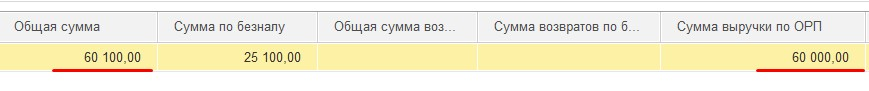
\includegraphics[width=1.0\textwidth]{12.jpg}
		\caption{<<Потерянный чек>>.}
		\label{ris:12.jpg}
	\end{figure}
	Здесь видно, что общая сумма  на 100 р. больше суммы выручки по ОРП.  (Рис.~\ref{ris:12.jpg})
	\item Первое, что  необходимо сделать - проверить по бумажным отчетом, что суммы внесены правильно. И если это действительно так и есть расхождения чисел, а не допущена ошибка ввода, приступаем к поискам потерянного чека.
	Нужно путем опроса кассиров или поиском в ОФД способом выяснить, какой товар был в этом чеке. . (Работа с сайтом ОФД изложена в п. \ref{5500})
	
	
	Установив товар в чеке или приняв решение чем его заменить нам нужно добавить этот чек в ОРП. Как  это сделать:
	
	\begin{itemize}
		\item Создать чек по нужной кассе. Записать его и с помощью ИТ отдела пересобрать ОРП.
		      Таким образом сумма выручки по ОРП сравняется с суммой по Z-отчету
	\end{itemize}
	
	
	
\end{itemize}

\newpage
%\subsection{Формирование документа Товарно-транспортная накладная ЕГАИС (входящая)}

\renewcommand{\arraystretch}{1.8} %% расстояние между строками таблицы
%\begin{landscape}
\begin{longtable}{|p{0.02\linewidth}|p{0.3\linewidth}|p{0.3\linewidth}|p{0.3\linewidth}|}
    %  {|c|c|l|c|}
    \hline
    № & \textbf{Действие} & \textbf{Ожидаемый результат} & \textbf{Фактический результат} \\
    %****************************************************************************************************
    \hline
    \hline
    \endhead
    \multicolumn{4}{|c|}{\textbf{\textit{******}}} \\
    \hline
    \hline

    %****************************************************************************************************


\end{longtable}	
%\newpage
\subsection{Формирование документа Возврат товаров поставщику}






\renewcommand{\arraystretch}{1.8} %% расстояние между строками таблицы
%\begin{landscape}
\begin{longtable}{|p{0.02\linewidth}|p{0.3\linewidth}|p{0.3\linewidth}|p{0.3\linewidth}|}
    %  {|c|c|l|c|}
    \hline
    № & \textbf{Действие} & \textbf{Ожидаемый результат} & \textbf{Фактический результат} \\
    %****************************************************************************************************
    \hline
    \hline
    \endhead
    \multicolumn{4}{|c|}{\textbf{\textit{Проверка на номенклатуру помеченную на удаление}}} \\
    \hline
    \hline
    \Rownum & Проверить, что включена константа <<крюПроверятьПомеченнуюНаУдалениеВДокументах>>  & &  \\
    \hline
    \Rownum &Перейти в раздел Закупки, выбрать <<Возвраты товаров поставщикам>>.  & 1. Открылся список документов  <<Возвраты товаров поставщикам>>;\par
    2. Отображаются все документы &  \\
    \hline
    \Rownum & Создать новый документ по кнопке \keys{Создать}  & 1. Открылась форма создания документа;\par
    2. По умолчанию в открывшейся форме заполнено поле <<Магазин>> &  \\
    \hline
    \Rownum & Заполнить реквизит <<Поставщик>> значением <<Метро>> &Заполнен <<Поставщик>> значением <<Метро>> ;    &  \\
    \hline
    \Rownum	& Нажать кнопку выбора складов & В форме выбора складов будет доступен только склад привязанный к текущему магазину  &  \\
    \hline
    \Rownum	& Выбрать склад & Заполнены реквизиты <<Склад>> и <<Организация>>  &  \\
    \hline
    \hline
    \Rownum	& Заполнить реквизит <<Причина возврата>> указав в качестве значения элемент выпадающего списка <<Возврат товара>> & Реквизит <<Причина возврата>> заполнен значением <<Возврат товара>> &  \\
    \hline
    \Rownum	& Нажать кнопку <<Добавить>> в табличной части <<Товары>>  & Откроется форма выбора справочника <<Номенклатура>>  &  \\
    \hline
    \Rownum	& Выбрать из справочника <<Номенклатура>> элемент помеченный на удаление & Заполнились поля в табличной части <<Код>>, <<Артикул>>, <<Номенклатура>>, <<Ед.изм>>, <<НДС>> &  \\
    \hline
    \Rownum	&Заполнить поле <<Количество>> значением <<1>>  & Заполнилось поле <<Количество>> &  \\
    \hline
    \Rownum	& Заполнить поле <<Цена>> значением <<1>>  & Заполнилось поле <<Цена>> &  \\
    \hline
    \Rownum	& Нажать кнопку \keys{Провести и закрыть} & 1. Программа выдает сообщение о неудачи проведения документа;\par 2. При закрытии окна сообщения в строке сообщений появляется текст ошибке с информацией, что документ содержит удаленную номенклатуру с указанием номеров строк и наименований &  \\
%****************************************************************************************************

%****************************************************************************************************

    %****************************************************************************************************

    %****************************************************************************************************
    \hline
    \hline
    \multicolumn{4}{|c|}{\textbf{\textit{Учет тары}}} \\
    \hline

    \hline
    \Rownum & Проверить, что включена константа <<крюПроводитьТару>>  & &  \\
    \hline
    \hline
    \Rownum &Перейти в раздел Закупки, выбрать <<Возвраты товаров поставщикам>>.  & 1. Открылся список документов  <<Возвраты товаров поставщикам>>;\par
    2. Отображаются все документы &  \\
    \hline
    \Rownum & Создать новый документ по кнопке \keys{Создать}  & 1. Открылась форма создания документа;\par
    2. По умолчанию в открывшейся форме заполнено поле <<Магазин>> &  \\
    \hline
    \Rownum & Заполнить реквизит <<Поставщик>> значением <<Метро>> &Заполнен <<Поставщик>> значением <<Метро>> ;    &  \\
    \hline
    \Rownum	& Нажать кнопку выбора складов & В форме выбора складов будет доступен только склад привязанный к текущему магазину  &  \\
    \hline
    \Rownum	& Выбрать склад & Заполнены реквизиты <<Склад>> и <<Организация>>  &  \\
    \hline
    \Rownum	& Заполнить реквизит <<Причина возврата>> указав в качестве значения элемент выпадающего списка <<Возврат кег>> & Реквизит <<Причина возврата>> заполнен значением <<Возврат кег>>  &  \\
    \hline
    \Rownum	& Нажать кнопку <<Добавить>> в табличной части <<Товары>>  & Откроется форма выбора справочника <<Номенклатура>>  &  \\
    \hline
    \Rownum	& Выбрать из справочника <<Номенклатура>> элемент с кодом <<00000013>> - <<КЕГ (50 л)>> & Заполнились поля в табличной части <<Код>>, <<Артикул>>, <<Номенклатура>>, <<Ед.изм>>, <<НДС>> &  \\
    \hline
    \Rownum	&Заполнить поле <<Количество>> значением <<1>>  & Заполнилось поле <<Количество>> &  \\
    \hline
    \Rownum	& Заполнить поле <<Цена>> значением <<1>>  & Заполнилось поле <<Цена>> &  \\
    \hline
    \Rownum	& Нажать кнопку \keys{Провести} &  Документ проводится без ошибок &  \\

    \hline
    \Rownum	& Выбрать команду <<Движения документа>> & Откроется отчет по движениям документа &  \\

    \hline
    \Rownum	& Найти в отчете движения по регистру <<Тара на складах>> & Движения документа по регистру накопления <<Тара на складах>> присутствуют. Измерения <<Период>>, <<Склад>>, <<Номенклатура>>, <<Поставщик>> заполнены. Значение ресурса <<Количество>> равно единице  &  \\
    \hline
    %****************************************************************************************************

    %****************************************************************************************************
    \hline
    \hline
    \multicolumn{4}{|c|}{\textbf{\textit{Очистка реквизита <<УчитыватьНДС>> и <<ЦенаВключаетНДС>>}}} \\

    \hline
    \Rownum & Проверить, что включена константа <<крюОчищатьНДСВВозвратеПоставщику>>  & &  \\

    \hline
    \Rownum &Перейти в раздел Закупки, выбрать <<Возвраты товаров поставщикам>>.  & 1. Открылся список документов  <<Возвраты товаров поставщикам>>;\par
    2. Отображаются все документы &  \\
    \hline
   \Rownum & Создать новый документ по кнопке \keys{Создать}  & 1. Открылась форма нового документа;\par
   2. По умолчанию в открывшейся форме заполнено поле <<Магазин>>\par
   3. Значение реквизитов <<ЦенаВключаетНДС>> и <<УчитыватьНДС>> на вкладке  <<Дополнительно>> равно <<Ложь>> &  \\
   \hline

    %****************************************************************************************************

     %****************************************************************************************************
    \hline
    \hline
    \multicolumn{4}{|c|}{\textbf{\textit{Печатная форма ТОРГ 12}}} \\
    \hline

    \hline
    \Rownum &Перейти в раздел Закупки, выбрать <<Возвраты товаров поставщикам>>.  & 1. Открылся список документов  <<Возвраты товаров поставщикам>>;\par
    2. Отображаются все документы &  \\
    \hline
    \Rownum & Открыть любой существующий документ  & 1. Открылась форма существующего документа;\par
     &  \\
     \hline
    \Rownum	& По кнопке выбора печатных форм выбрать <<ТОРГ-12(Товарная накладная на возврат)>>  & Сформировалась печатная форма &  \\
    \hline
    \Rownum	& Проверить представление организации и поле <<Вид операции>> в шапке & 1. В представлении организации присутствует КПП организации\par
    2. Поле <<Вид операции>> заполнено значением <<Возврат>>  &  \\


    %****************************************************************************************************





    \hline
    \Rownum	& test &  &  \\ %\nopagebreak Для запрещения разбиения страниц применяется команда \nopagebreak сразу после двух слешей в конце строчки.
    \hline
\end{longtable}
\newpage

%\section{Справочники}
%\marginnote{\Date{Ср.}{08}{Апр.}{2020}}[-20pt]
\subsection{Номенклатура}

\begin{itemize}
	\item Изменение группы справочника "Номенклатура" блокируется в зависимости от установленной константы "крюИспользоватьБлокировкуНоменклатуры" и установки прав в РегистрСведений "крюПраваПользователей" (расш.)
	\Nameref{503}
	\item Изменение элемента справочника  "Номенклатура" блокируется в зависимости от установленной константы "крюИспользоватьБлокировкуНоменклатуры" и установки прав в РегистрСведений
	"крюПраваПользователей" блокируется не вся форма, а по определенному списку реквизитов и элементов управления
	(расш.) \Nameref{503}
	\item Блокировка реквизита "Артикул" вынесена отдельно и управляется константой "крюБлокироватьАртикул" 
	(расш.) \Nameref{503}	
\end{itemize}

\subsection{Организации}

\begin{itemize}

	\item Изменение элемента справочника  "Организации" блокируется при открытии в зависимости от установки прав в РегистрСведений "крюПраваПользователей" 
	(расш.) \Nameref{506}
	
\end{itemize}


\subsection{ФизическиеЛица}

\begin{itemize}
	
	\item Изменение элемента справочника  "Физические лица" блокируется при открытии в зависимости от установки прав в РегистрСведений "крюПраваПользователей" 
	(расш.) \Nameref{507}
	
\end{itemize}


\subsection{СтатьиДвиженияДенежныхСредств}

\begin{itemize}
	
	\item Изменение элемента справочника  "Статьи движения денежных средств" блокируется при записи в зависимости от установки значения константы "крюБлокироватьДДС" 
	(расш.) \Nameref{508}
	
\end{itemize}

 % Обработка по контролю минимальных остатков ключевых позиций
%\newpage
%\subsection{Описание прочих изменений в конфигурации}
\marginnote{\Date{Пт.}{30}{Июня}{2017}}[20pt]
\subsubsection{Показ остатков в кассе}
\begin{itemize}	
	\item При выборе на кассе кличества товара большего чем есть на остатках выводилось сообщение оп превышении остатка с не хватающим количеством, что позволяло косвенным образом узнать остаток товара на складе.\par
	Сообщение изменено, количество недостающего товара не показывается.
\end{itemize}	
\subsubsection{Контроль движения возвратной тары}	 
\begin{itemize}	
	\item Возвратная тара теперь может двигаться только документами "<Поступление товаров"> и "<Возврат товаров поставщику">. При наличии возвратной тары  в табличной части "<товары"> других документов, эти документы не проводятся.  
\marginnote{\Date{Чт.}{27}{Июля}{2017}}[20pt]	
	\item Добавлена константа "<крюДатаНачалаУчетаКег"> для того, что бы документы более ранней даты при перепроведении не делали движения по регистру "<Тара на складах">.  
\end{itemize}			


%	\begin{figure}[H]
%		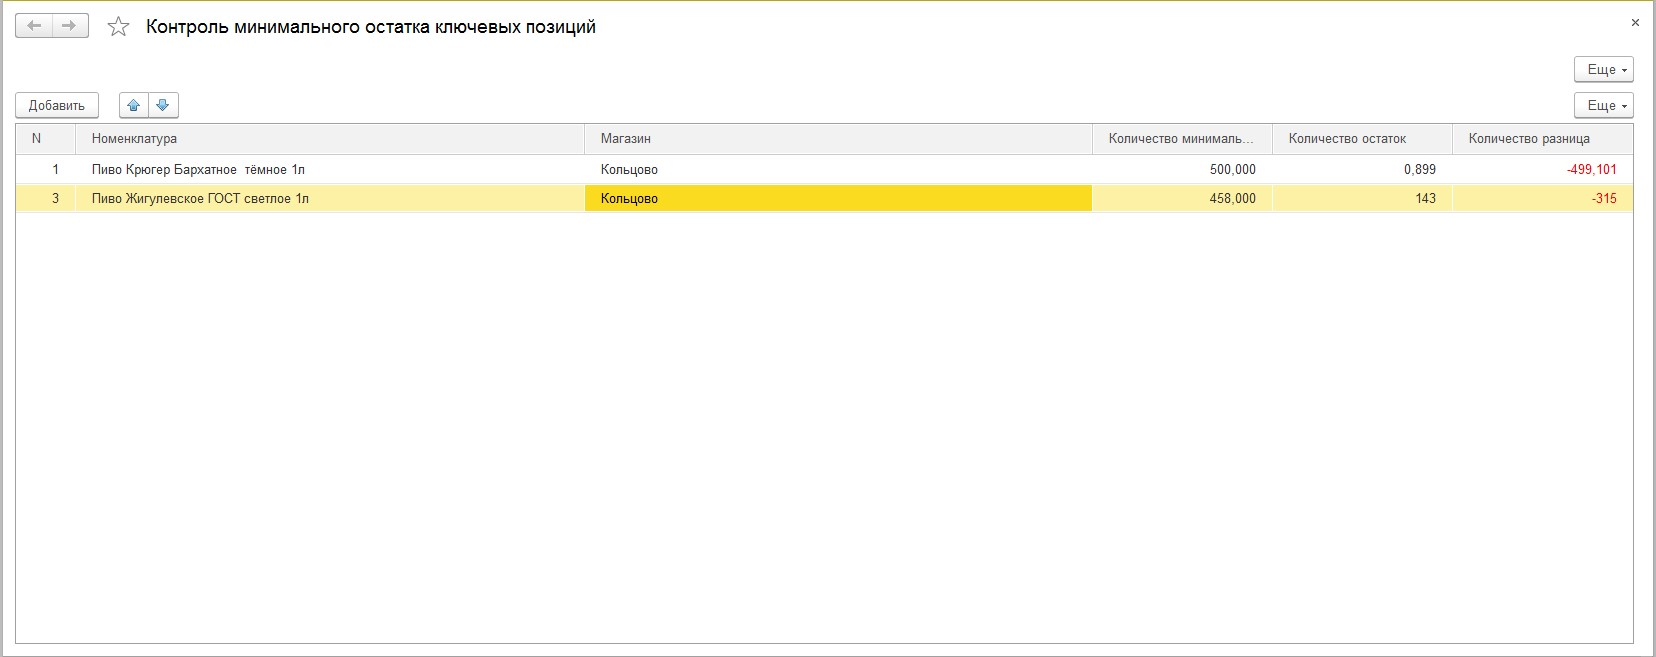
\includegraphics[width=0.90\textwidth]{10_1.jpg}
%		\caption{Старт при запуске системы.}
%		\label{ris:10_1.jpg}
%	\end{figure}

 % Описание прочих изменений
%\newpage

\listoffigures	
%\newpage

%\addcontentsline{toc}{chapter}{Index}	

\newpage

%\printglossary



\begin{versionhistory}
	\vhEntry{0.01}{11.05.20}{PK}{Добавлены схемы}
    \vhEntry{0.10}{11.05.20}{PK}{Добавлено описание и настройка}
    \vhEntry{0.20}{11.05.20}{PK}{Добавлено описание расширений}
    \vhEntry{0.25}{13.05.20}{PK}{Расширено описание}

\end{versionhistory}
%\vhListAllAuthorsLong % Список авторов
%\newpage
%\listoftodos
%\printindex
%\listoftodos[Необходимые правки]
\end{document}
